%%%%%%%%%%%%%%%%%%%%%%% file SelHex_proceedings.tex %%%%%%%%%%%%%%%%%%%%%%%%%

\documentclass[proc]{edpsmath}

%%%%%%%%%%%%%--PREAMBLE--%%%%%%%%%%%%%%%%%%
%%-----------------------------
%%         ...........
%%         your macros
%%         ...........
%%-----------------------------
\usepackage{tikz}
\usepackage{cases}
\setcounter{MaxMatrixCols}{20}

%
%\newtheorem{theorem}{Theorem}[section]
%\newtheorem{algo}[theorem]{Algorithm}
%\newtheorem{definition}{Definition}[section]
%\newtheorem{remark}[theorem]{Remark}

%%%%%%%%%%%%%%%--BODY--%%%%%%%%%%%%%%%%%%

\begin{document}
\selectlanguage{english}

%%-----------------------------
%%      the top matter
%%-----------------------------
\title{Solving the Guiding-Center model\\on a regular hexagonal mesh}%\thanks{...}\thanks{...}% At most 5 thanks
%
\author{Michel Mehrenberger} \address{IRMA, Universit\'e de Strasbourg, 7, rue Ren\'e Descartes, 67084 Strasbourg \& INRIA-Nancy Grand-Est, projet TONUS, 
\email{mehrenbe@math.unistra.fr}}
\author{Laura S. Mendoza} \address{Max-Planck-Institut f\"{u}r Plasmaphysik, Boltzmannstr. 2, D-85748 Garching bei M\"unchen, Germany. \email{mela@ipp.mpg.de\ \&\ sonnen@ipp.mpg.de}} 
\secondaddress{Technische Universit\"at M\"unchen, Boltzmannstr. 3, D-85748 Garching, Germany.}
\author{Charles Prouveur}\address{Universit\'e de Lyon, UMR5208, Institut Camille Jordan,
43 boulevard 11 novembre 1918, F-69622 Villeurbanne cedex, France}
\author{Eric Sonnendr\"{u}cker}\sameaddress{2,3}
%
%\dedicated{\it Dedicated to Maurice Dupont} %if necessary
%


%%-----------------------------
%%          Abstract
%%-----------------------------
%% English version ............
\begin{abstract} 
This paper introduces a Semi-Lagrangian solver for the Vlasov-Poisson equation on a regular hexagonal mesh. The latter is composed of equilateral triangles, thus it doesn't contain any singularities, unlike polar meshes. We focus on the guiding-center model. Thus, a Poisson solver for the hexagonal mesh is developed. For the interpolation step of the Semi-Lagrangian scheme, a comparison is made between using box-splines and Hermite finite elements. We expect to adapt it to more complex models and geometries.
\end{abstract}

%% French version ............
\begin{resume} 
Dans cet article nous introduisons un solveur semi-Lagrangien pour l'\'equation de Vlasov-Poisson sur un maillage hexagonal r\'egulier. Ce dernier est compos\'e de triangles \'equilat\'eraux, ainsi il ne pr\'esente aucune singularit\'e, contrairement au maillage polaire. Nous nous concentrons ici sur le mod\`ele centre-guide. \`A cette fin nous avons d\'evelopp\'e un solveur de l'\'equation de Poisson pour maillage hexagonal. Au regard de l'interpolation, nous comparons les r\'esultats obtenus avec des \'el\'ements finis d'Hermite et des box-splines.   Dans l'avenir, ce code sera adapt\'e \`a des g\'eom\'etries et mod\`eles plus complexes.  
\end{resume}


%% Making the title ..........
\maketitle


%%-----------------------------
%%      Introduction
%%-----------------------------
\section*{Introduction}


There are three kinds of regular pavings of the plane: using squares, triangles or hexagons. When considering meshes, the dual mesh of a square mesh is a shifted square mesh and the regular triangle mesh is the dual of the regular hexagonal mesh.

In magnetic fusion applications the embedded magnetic flux surfaces play an important role and introduce an important anisotropy\cite{Angelino2009}. For this reason one gets favourable numerical properties when grid points align on the concentric magnetic flux surfaces. When trying to do this with a mapped cartesian grid, one ends up with a polar coordinates mesh (when the flux surfaces are circles) or something topologically equivalent. This yields smaller and smaller cells when getting closer to the center as well as a singularity at the center. This is numerically far from optimal. 

Different strategies have been implemented to avoid these singularities, we can cite among others: the isoparametric analysis approach done by J. Abiteboul et al. \cite{abiteboul2011solving} and A. Ratnani \cite{ratnani2011isogeometric} or N. Besse and E. Sonnendr\"{u}cker's work with non-structured meshes\cite{Besse2003341}. The works presented on these papers are particularly interesting as not only they avoid singularities but they are also extremely flexible and can be easily adapted to more complex geometries. However, even if the approach is different in every paper, some limitations are the numerical complexity, the advection of the derivatives and, the localisation of the feet of the characteristics. 
A recent study was made by T. Nguyen et al.\cite{axioms3020280} to compare different Poisson solvers on the disk. 

Tiling a regular hexagon into triangles yields a mesh of equilateral triangles having all the same area\cite{Sadourny1968}. This grid can be easily mapped to a circle by slightly stretching the edges of the hexagon. This yields a nice mesh of a disk with slightly stretched triangles of almost the same size and there is no singularity in any point of the domain. 
Additionally, such a mesh has a clear structure with three privileged directions, thus it is completely straightforward to localise points within this mesh. The derivatives along the three directions can also be nicely computed using finite differencing along uniform lines. 
And last but not least, there is a spline construction on this mesh, called box-spline \cite{Condat2008}. These splines have a hexagonal support and are invariant by translations along the three directions of the mesh. 

The disadvantages previously mentioned, are not present when dealing with the simple and straightforward hexagonal mesh. Regarding the computational efficiency, all our simulations include an analysis and comparison with more common methods. Lastly, we suggest this scheme as an introduction to treat more complex geometries. Indeed by a simple mapping it will be easy to work with curvilinear coordinates.

In this work, we focus on adapting the Semi-Lagrangian scheme to this hexagonal mesh. This scheme consists basically of two steps: computing the characteristics' origins and interpolating at these points. For the latter, we compare two different approaches: one using box-splines and the second approach using Hermite Finite Elements. Both interpolation methods, as well as the mesh, are presented in section~\ref{sec:interpolation}. In section~\ref{sec:poisson_eqn}, we present a Poisson solver adapted to the hexagonal mesh. We present a guiding-center approximation of the 2D Vlasov Poisson system\cite{Golse1998865}, and the Semi-Lagrangian scheme to solve it, in section~\ref{sec:BSL_scheme}. Finally, in section~\ref{sec:results} we compare the results of the scheme using box splines with the ones using Hermite finite elements, we also compare them to more traditional meshes, such as the polar mesh. Besides the guiding-center model, different advection models have been simulated in this section.


%%-----------------------------
%% Interpolation 
%%-----------------------------
\section{Interpolation on regular hexagonal mesh}
\label{sec:interpolation}
%%-----------------------------
\subsection{The hexagonal mesh}

The hexagonal mesh is obtained by tiling a regular hexagon into equilateral triangles. The mesh obtained can be generated by three vectors. These unit vectors are

\begin{equation}
	\mathbf{r_1} = \begin{pmatrix}\sqrt{3}/2 \\  1/2
		\end{pmatrix} ~~~~~~~~
	\mathbf{r_2} = \begin{pmatrix}-\sqrt{3}/2 \\ 1/2
		\end{pmatrix} ~~~~~~~~
	\mathbf{r_3} = \begin{pmatrix} 0 \\ 1
		\end{pmatrix}
\end{equation}

The 2D lattice sites are obtained by the product $\mathbf{Rk}$ where $\mathbf{R} = [\mathbf{r_1 r_2}]$ and $\mathbf{k} = [k_1, k_2]^T \in \xZ$.  To obtain exactly the mesh as in Figure \ref{fig:hexmesh}, we need to define a few extra parameters : an origin -- denoted $P_0(x_0, y_0)$, a radius $L$ which is the distance between the origin and an external node and the number of cells $N_c$ on any radius.


\begin{figure}[h!]
	\begin{center}
	\begin{tabular}{ccc}
	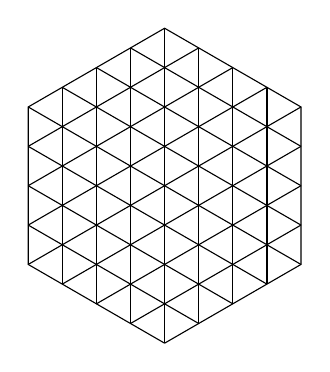
\begin{tikzpicture}
		% Three directions of grid
		% vertical direction
		\draw (0,-2) -- (0,2);
		\draw (-0.433,-1.75) -- (-0.433,1.75);
		\draw (-0.866,-1.5) -- (-0.866,1.5);
		\draw (-1.3,-1.25) -- (-1.3,1.25);
		\draw (0.433,-1.75) -- (0.433,1.75);
		\draw (0.866,-1.5) -- (0.866,1.5);
		\draw (1.3,-1.25) -- (1.3,1.25);

		% upward
		\draw(-1.732,-1) -- (1.732,1);
		\draw (-1.732,-.5) -- (1.3,1.25);
		\draw (-1.732,0) -- (.866,1.5);
		\draw (-1.732,.5) -- (.433,1.75);
		\draw (-1.3,-1.25) -- (1.732,.5); 
		\draw (-0.866,-1.5) -- (1.732,.0);
		\draw (-0.433,-1.75) -- (1.732,-.5);
		% downwards
		\draw(-1.732,1) -- (1.732,-1);
		\draw (-1.732,.5) -- (1.3,-1.25);
		\draw (-1.732,0) -- (.866,-1.5);
		\draw (-1.732,-.5) -- (.433,-1.75);
		\draw (-1.3,1.25) -- (1.732,-.5); 
		\draw (-0.866,1.5) -- (1.732,.0);
		\draw (-0.433,1.75) -- (1.732,.5);
		% Hexagog
		\draw (0,-2) -- (1.732,-1) -- (1.732,1) -- (0,2) -- (-1.732,1) -- (-1.732,-1) -- (0,-2) ; 
	\end{tikzpicture}
	& ~~~~~~~~ &
	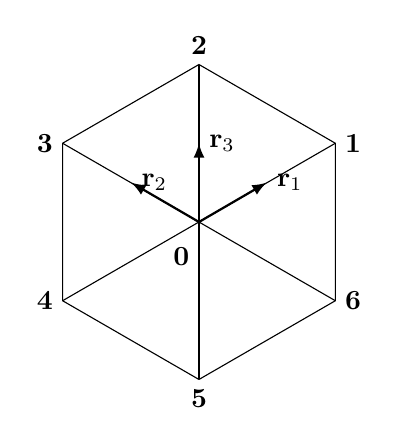
\begin{tikzpicture}
		% Three directions of grid
		% vertical direction
		\draw(0,-2) -- (0,2) node[pos = 0.45, below left]{$\mathbf{0}$};
		\draw[-latex,thick](0,0)--(0,1)node(yline)[right]{$\mathbf{r}_3$};
		\draw[-latex,thick](0,0)--(0.86,.5)node(yline)[right]{$\mathbf{r}_1$};
		\draw[-latex,thick](0,0)--(-0.86,.5)node(yline)[right] {$\mathbf{r}_2$};		
		\draw(-1.732,-1) -- (1.732,1);
		\draw(-1.732,1) -- (1.732,-1);
		\draw (0,-2) node[below]{$\mathbf{5}$} -- (1.732,-1) node[right]{$\mathbf{6}$} -- (1.732,1) node[right]{$\mathbf{1}$} -- (0,2) node[above]{$\mathbf{2}$}-- (-1.732,1) node[left]{$\mathbf{3}$} -- (-1.732,-1) node[left]{$\mathbf{4}$} -- (0,-2) ; % size 2
	\end{tikzpicture}
	\end{tabular}
	\end{center}
	\caption{The hexagonal lattice and the vectors $\mathbf{r_1, r_2, r_3}$ that generate such a mesh}
  \label{fig:hexmesh}
\end{figure}


The mesh is based on uniform hexagons of the first type (see \cite{Ulichney87}). For local and global notations we will use the following convention : the point at the center will be the point of index $0$. Following the direction $\mathbf{r_1}$ the next point will be indexed $1$, and the notations will follow in a counter-clockwise motion. And so on, until all the points of the domain have been indexed. See Figure \ref{fig:hexmesh}. We will denote $H_i$ the unit hexagon cell that is centred at the point of global index $i$.

Besides the fact that the hexagonal mesh contains no singularities, its regularity allows us to localise effortlessly the characteristic's origin for the Semi-Lagrangian scheme. Nevertheless, the accuracy of the method depends heavily on the interpolation method chosen. For example, for a cartesian grid, it is common to use cubic splines which have shown to give accurate results in an efficient manner (\textcolor{red}{see [look for a ref]}). In our problem, with the hexagonal lattice, B-splines do not exploit the isotropy of the mesh (for more information see \cite{Mersereau79-IEEE}) and are defined by a convolution on 2D, which cannot be done for our mesh. Therefore, we need to use another approach. On the following two sub-sections we present two different strategies: one using box splines and a second one using Hermite Finite Elements.


%%-----------------------------
\subsection{Box Splines quasi-interpolation}

There are mainly two splines' families that take advantage of the geometry's properties : hex-splines and the three directional box-splines. For a detailed comparison between these two types of splines we will refer to \cite{Condat2007}. Based on the latter, we have chosen to use box splines, as the results are more stable. And lastly, also based on the previously cited paper, we decide to use a quasi-interpolation method.

%%..............................
\subsubsection{Box-Splines: General Definition}

Box-splines are a generalisation of the more known splines' family: B-splines. They are also piecewise polynomial and they share some properties, such as: compact support, positiveness, symmetry and partition of unity. But, unlike B-splines, box-splines are defined from a generator matrix $\Xi$. Therefore, to construct them on the hexagonal lattice, we will use the generator vectors $\mathbf{r_1, r_2, r_3}$. The general definition is \cite{Boor1993, Condat2006}:

\begin{dfntn}[Box-splines]

	Let $\Xi$ be a $d \times m$ matrix with non-null columns in  $\xR^d$. A box-spline $\chi_\Xi$ associated to the matrix $\Xi$, is a multivariate function $\chi_\Xi : \xR^d \longrightarrow \xR$. If $\Xi$ is a square invertible matrix, \emph{i.e.} when $m = d$ and $\det(\Xi) \neq 0$, we define a box spline with the formula below
	\begin{equation}
		\chi_{\Xi} (\mathbf{x}) = \left\{
  		\begin{array}{l l}
    		\dfrac{1}{\lvert \det(\Xi)\rvert} & \quad \text{if $\Xi^{-1}\mathbf{x} \in [0,1)^2$ }\\
    		0 & \quad \text{otherwise}
  		\end{array} \right.
	\end{equation}

	If $\Xi \cup \mathbf{v}$ is a $d \times (m + 1)$ matrix, composed by the $m$ columns vectors from $\Xi$ to which we append the vector $\mathbf{v}$, we define the box-spline $\chi_{\Xi \cup \mathbf{v}}$ by recursion:

	\begin{equation} 
	\label{eqn:boxsplines_basis}
		\chi_{\Xi \cup \mathbf{v}}(\mathbf{x}) = \int_0^ 1 \chi_\Xi(\mathbf{x}-t\mathbf{v})dt
	\end{equation}

\end{dfntn}

\rmrk The box-splines can have different degrees in each direction. Thus, there are different definitions of the degree. We will adopt the definition below.

\begin{dfntn}[Degree of a Box-spline]
Let $\Xi$ be a $d \times d$ matrix with non-null columns in $\xR^d$. The column vectors of $\Xi$ form a generating basis of $\xR^d$ and are linearly independent. Then, the box-spline of degree $N$ of generating matrix $\Xi$, $\chi^N_\Xi$, is the box-spline associated to $\Xi$, where all the generating vectors have multiplicity $N+1$. This yields, that $\chi^N_\Xi$ is piecewise polynomial of degree $N$.


\end{dfntn}

\begin{figure}[h!]
	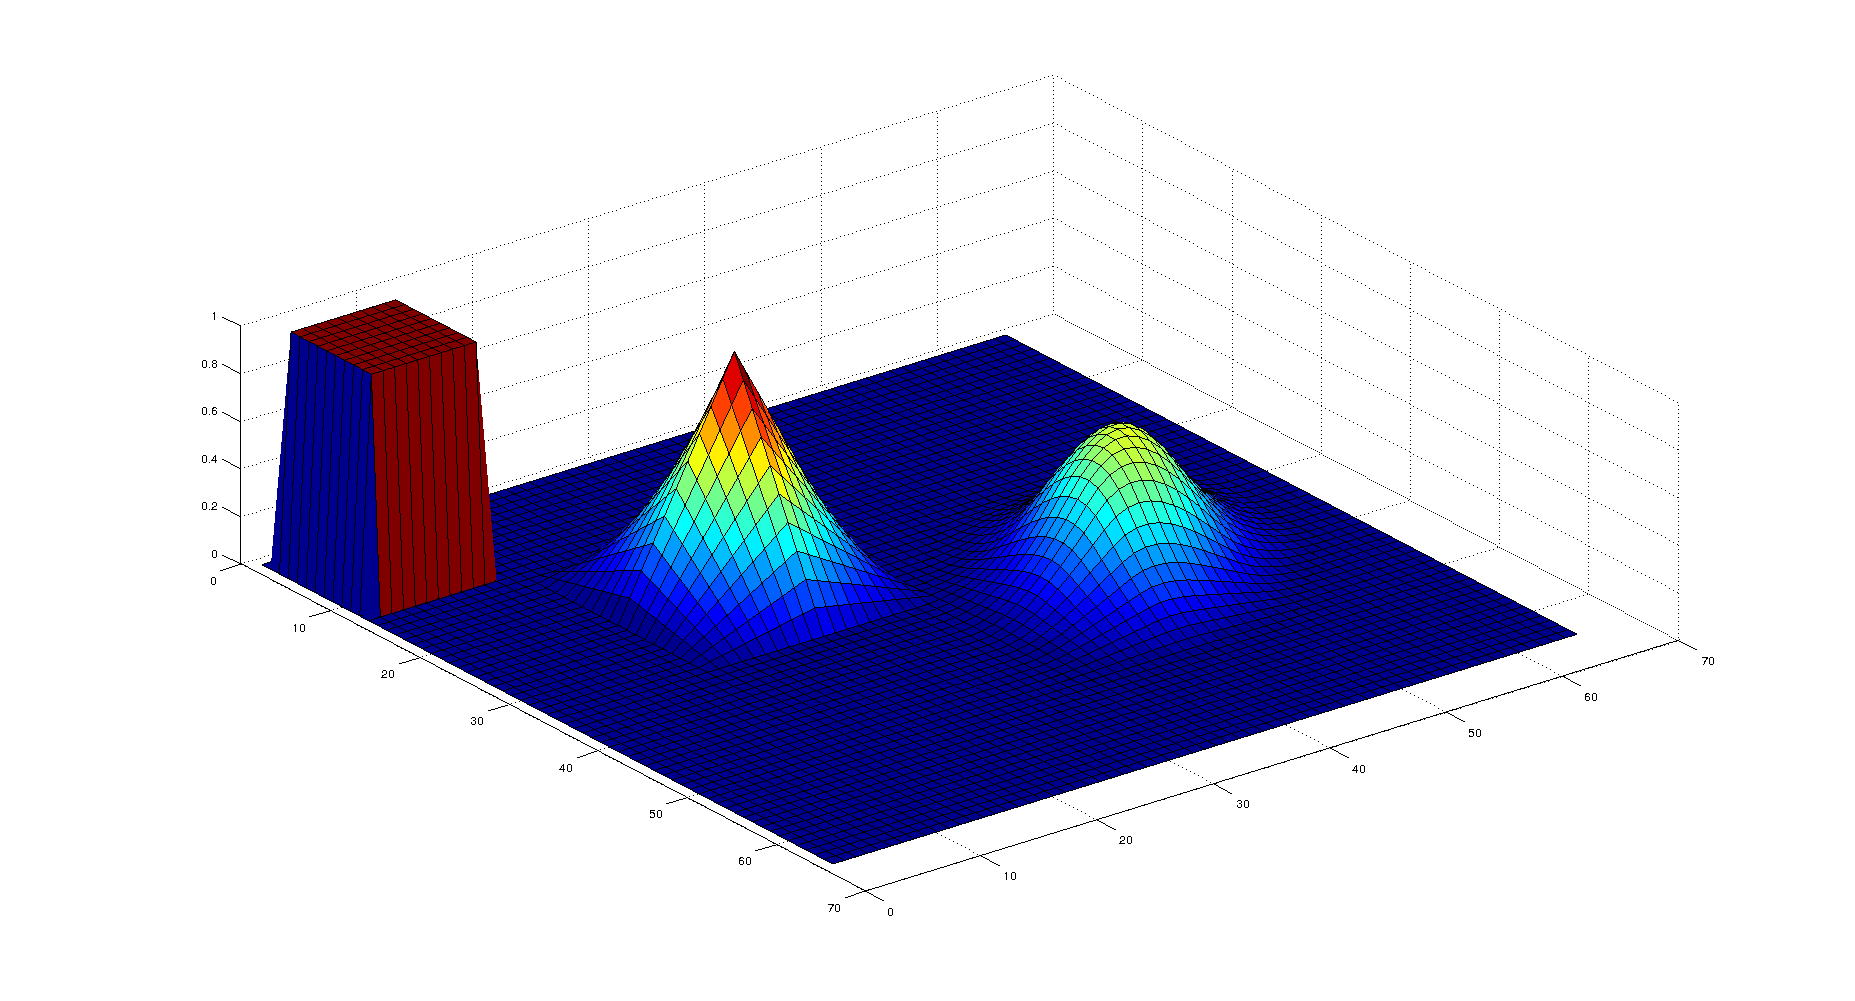
\includegraphics[scale=0.15]{figures/boxsplines3d.png}
	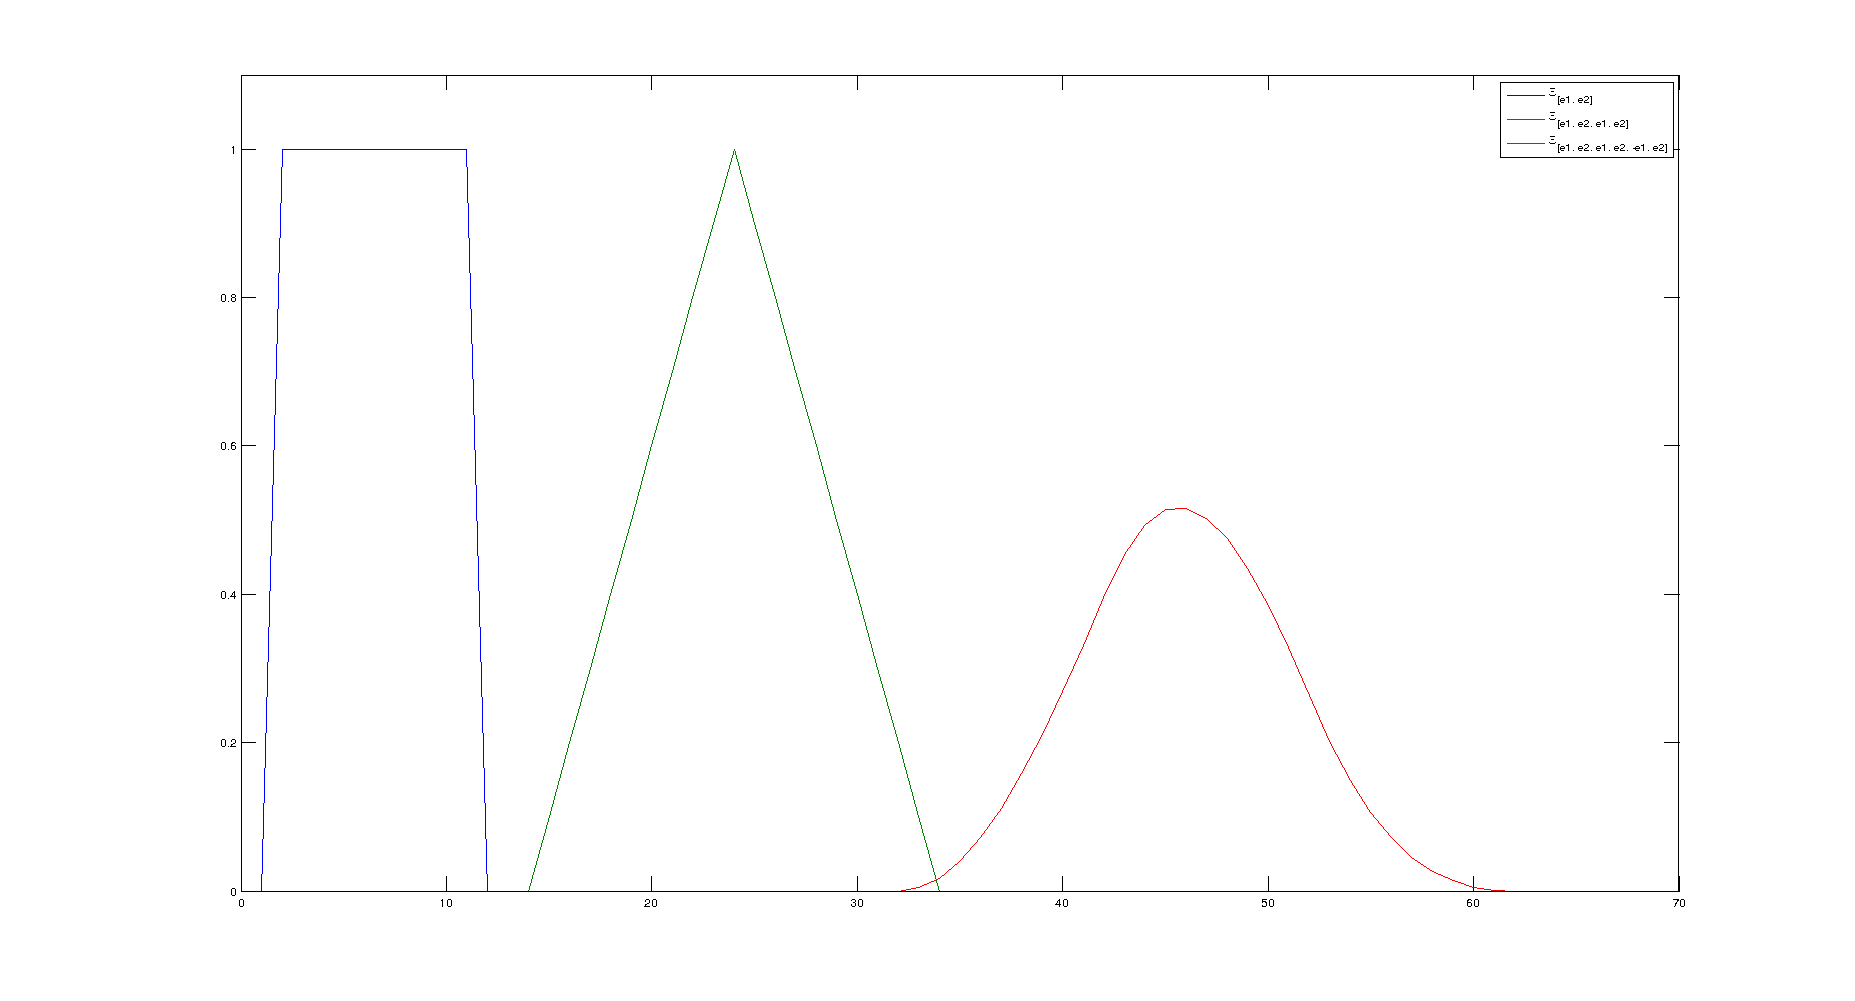
\includegraphics[scale=0.15]{figures/boxsplines2d.png}
	\caption{On the left: Box splines representation of $\Xi_[e_1, e_2]$, $\Xi_[e_1, e_2, e3]$, and $\Xi_[e_1, e_2, e_3, e_4]$. Where $e_1 = ( 0, 1 )^T$ , $e_2 = ( 1, 0)^T$, $e_3 = e_1 + e_2$, and $e_4 = e_1 - e_2$. On the right: the 2d projection of the box-splines to the $x$ plane.}
	\label{fig:boxsplines3d}
\end{figure}

	


%%..............................
\subsubsection{The quasi-interpolation scheme}

Let us describe the method: we are given an initial sample $s[\mathbf{k}] = f_0(\mathbf{R} \mathbf{k})$, where the points $\mathbf{R} \mathbf{k}$ belong to our hexagonal mesh, and we need to know the values $f(\mathbf{x})$ where $\mathbf{x} \notin \mathbf{R} \mathbf{k}$. We want a spline surface $f(\mathbf{x}) = \sum c[\mathbf{k}] \chi^N(\mathbf{x} - \mathbf{R}\mathbf{k})$, where $\chi^N$ are the box-splines of degree $N$ of matrix $\mathbf{R}$ and $c[\mathbf{k}]$ are the coefficients associated to them. The reconstruction is defined such that $f(\mathbf{x})$ approximates $f_0(x)$ to a certain order $N$ or, in other words, the approximation is exact only if $f_0(x)$ is a polynomial of degree $N-1$ or less. This is different to the classic interpolation method, where the reconstruction is exact on mesh points in any case. The $c[\mathbf{k}]$ coefficients are the box-splines coefficients, to compute them we cannot longer solve a matrix-vector system because of the extra degree of freedom given by the quasi-interpolation method. Thus, the  $c[\mathbf{k}]$ coefficients are obtained by discrete filtering\cite{Condat2006a}

\begin{equation}
\label{eqn:coefs}
 c = s * p
\end{equation}

where $*$ is the convolution operator, $s$ is the initial sample data and $p$ is a pre-filter which will be defined later on.


\subsubsection{Box splines coefficients}

How we determine the splines coefficients is almost as important as the splines themselves. We recall we have the formula \eqref{eqn:coefs}. Based on the literature available (notably \cite{Condat2007}) we have chosen for second-order box-splines the quasi-interpolation pre-filters $p_{IIR2}$ which seem to give better results within a competitive time. The pre-filter $p_{IIR2}[i]$ of the point of local index $i$, for splines of order 2, is defined as follows : 


\begin{equation}
\label{eqn:filterIIR2}
p_{IIR2} [i] = \left\{
  \begin{array}{l l}
    1775/2304\text{,} & \quad \text{if } i = 0\\
    253/6912\text{,} & \quad \text{if } 0<i<7\\
    1/13824\text{,} & \quad \text{if } 6<i<19 \text{ and $i$ odd}\\
    11/6912\text{,} & \quad \text{if } 6<i<19 \text{ and $i$ even}\\
    0 & \quad \text{otherwise}
  \end{array} \right.
\end{equation}

%Or for the splines of order 3 :
%
%\begin{equation}
%\label{eqn:filterIIR3}
%p_{IIR2} [i] = \left\{
%  \begin{array}{l l}
%    244301/460800\text{,} & \quad \text{if } i = 0\\
%    42269/576000\text{,} & \quad \text{if } 0<i<7\\
%    -11809/6912000\text{,} & \quad \text{if } 6<i<19 \text{ and $i$ odd}\\
%    1067/144000\text{,} & \quad \text{if } 6<i<19 \text{ and $i$ even}\\
%    -23/576000\text{,} & \quad \text{if } 18<i<37 \text{ and ($k_1 = 0$ or $k_2 = 0$ or $k_1 = k_2$) }\\
%    -109/288000\text{,} & \quad \text{if } 18<i<37 \\
%    	-1/13824000\text{,} & \quad \text{if } 36<i<61 \text{ and ($k_1 = 0$ or $k_2 = 0$ or $k_1 = k_2$) }\\
%    	97/6912000\text{,} & \quad \text{if } 36<i<61 \text{ and ($|k_1| = 2$ or $|k_2| = 2$) }\\
%    	1/576000\text{,} & \quad \text{if } 36<i<61\\    		
%    0 & \quad \text{otherwise}
%  \end{array} \right.
%\end{equation}

For higher orders, we refer to the previously mentioned papers.

\subsubsection{Optimizing the evaluation}

At the present state we have all the elements for the approximation of a function $f$ with second order box-splines

\begin{equation}
\tilde{f}(\mathbf{x}) = \sum_{\mathbf{k} \in \xZ^2} c[\mathbf{k}] \chi^2(\mathbf{x} - \mathbf{R}\mathbf{k})
\end{equation}

Even if we limit our sum to the vector $\mathbf{k}$ that defines our domain, we would like to take advantage of the fact that the splines $\chi^1$ are only non-zeros in a limited number of points. Therefore we need to know the indices $\mathbf{k}$ such that $\chi^1(\mathbf{x} - \mathbf{R} \mathbf{x}) \neq 0$. For this purpose we will use the strategy suggested in \cite{Condat2007} : to start we need to obtain the indices on the coordinate system generated by $\mathbf{R}$ : $\mathbf{k}_0 = \left[ \lfloor u \rfloor \; \lfloor v \rfloor \right]$ where $\left[ u \; v \right]^T = \mathbf{R}^ {-1} \mathbf{x} $. Thus, in our case, with splines $\chi^2$ we only need 4 terms associated to the encapsulating rhomboid's vertices : $\mathbf{R}\mathbf{k}_0$, $\mathbf{R}\mathbf{k}_0 + \mathbf{r_1}$, $\mathbf{R}\mathbf{k}_0 + \mathbf{r_2}$ and $\mathbf{R}\mathbf{k}_0 + \mathbf{r_1} + \mathbf{r_2}$. Finally we obtain :

\begin{align}
\label{eqn:chi2_fct_interpol}
\tilde{f}(\mathbf{x}) =& \;\;\;\;\; c[\mathbf{k}_0] \; \chi^1(\mathbf{x} - \mathbf{R}\mathbf{k}_0) \nonumber\\
	&+ c[\mathbf{k}_0 +[1,0]]\; \chi^1(\mathbf{x} - \mathbf{R}\mathbf{k}_0 - \mathbf{r_1}) \nonumber\\
	&+ c[\mathbf{k}_0 +[0,1]]\; \chi^1(\mathbf{x} - \mathbf{R}\mathbf{k}_0 - \mathbf{r_2}) \nonumber\\
	&+ c[\mathbf{k}_0 +[1,1]]\; \chi^1(\mathbf{x} - \mathbf{R}\mathbf{k}_0 - \mathbf{r_1} - \mathbf{r_2})
\end{align}

\rmrk  As the $\chi^1$ spline has a support of radius the unity, one of the elements of \eqref{eqn:chi2_fct_interpol} is null. But this formula allows us to keep a short general formula for all points on the mesh without having to compute the indices of the cell to which $\mathbf{x}$ belongs to.

\rmrk For the box-splines of degree $2$, there are $12$ coefficients to compute (see Figure~\ref{fig:SL_hex}). Numerically, we can take the encapsulating rhomboid of edge length $3$ (instead of 1). Thus, the number of null terms for the interpolation with $\chi^2$ is $4$.

%%-----------------------------
\subsection{Hermite Finite Elements interpolation}

Another family of finite elements used to interpolate is the Hermite's one.
To interpolate at a point X of barycentric coordinates $(\lambda_1,\lambda_2,\lambda_3)$ in the triangle T of vertices $S_1$, $S_2j$, and $S_3$, we need a finite element with a local interpolation operator $\Pi_T $. This operator can be defined with the product of a set of degrees of freedom $\Sigma_T$ with a set of basis functions $\Xi$ which depends on the barycentric coordinates.\\
For this part we define the indices i, j and k with the following relations:
\begin{equation*}
j=i[3]+1 ~,~ k=j[3]+1.
\end{equation*}  
Here $i[3]$ (respectively $j[3]$) is the rest of the euclidean division of $i$ (resp. $j$) by $3$.\\

Several elements have been tested here:
The Z2 and Z3 Zienkiewicz elements, the Hsieh-Clough-Tocher reduced (HCT-r) and complete (HCT-c), and the Ganev-Dimitrov element. These elements can be found in \cite{z} and \cite{b1} . Here we show specifically how the hexagonal structure simplifies the interpolation with these elements.\\

\subsubsection{The Z2 and Z3 Zienkiewicz elements}
Z2 approach uses 9 degrees of freedom which are the values at the vertices of the triangle and the values of the derivatives in the direction of the edges at every vertex.
\begin{equation*}
 \Sigma_T = \lbrace \forall i \in [|1;3|], f(S_i),\partial_x(S_i),\partial_v(S_i) \rbrace 
\end{equation*}

 \noindent Z3 uses one more degree of freedom which is the value at the center of the triangle:
\begin{equation*}
 \Sigma_T = \lbrace \forall i \in [|1;3|], f(S_i),\partial_x(S_i),\partial_v(S_i); f(C) \rbrace 
\end{equation*}

 \noindent The advantage of using the Z3 element is the gain of one order of precision with an order 3 instead of an order 2 for the Z2 approach. Let us note that although adding one degree of liberty seems harmless enough, the center points for a hexagonal mesh represents a computional cost multiplied by 3. Indeed they are  2 times more centers than vertices. Therefore the number of points which must be computed is tripled. 
 
Let us define the basis functions needed to interpolate with the element Z2 : 
\begin{equation*}
\phi = \lambda_1 \lambda_2 \lambda_3 
\end{equation*}
\begin{equation*}
\xi _i= \lambda_i^3 - \phi ~\text{and}~ \xi_{ij}= \lambda_{i}^2 \lambda_j + \frac{\phi}{2} 
\end{equation*}
\begin{equation*}
\phi_i = 3\lambda_{i}^2 -2 \xi_i ~\text{and} ~\phi_{ij} = h_{ij} \xi_{ij}=h \xi_{ij}
\end{equation*}


\noindent $\phi_i$ is the basis function associated with the value of the function at $S_i$ while $\phi_ij$ are associated with the derivatives in the direction of the edges.    
The fact that T is equilateral is exploited here by replacing $h_{ij}$ with h since the length of $ [S_iS_j]$ is constant. Finally for Z2 we have :
\begin{equation*}
 \Pi (X) = \sum \limits_{\substack{i=1 }}^{3}{ [f(S_i).\phi_i + \sum \limits_{\substack{j\neq i }}^{}{ \frac{\partial f(S_i)}{\partial  \overrightarrow{ S_i S_j } }.\phi_{ij} } ] } 
\end{equation*}

\noindent In the same manner, let us define the basis functions needed to interpolate with Z3: 
\begin{equation*}
\phi_i = 3\lambda_{i}^2 -2 \xi_i - 9 \phi
\end{equation*}
\begin{equation*}
\phi_{ij} = h_{ij} (\xi_{ij} -\frac{3}{2}\phi)=h (\xi_{ij} -\frac{3}{2}\phi)
\end{equation*}
\begin{equation*}
\phi_{123}=27\phi
\end{equation*}

\noindent therefore for $Z_3$ we have :
\begin{equation*}
 \Pi (X) = \sum \limits_{\substack{i=1 }}^{3}{ [f(S_i).\phi_i + \sum \limits_{\substack{j\neq i }}^{}{ \frac{\partial f(S_i)}{\partial  \overrightarrow{ S_i S_j } }.\phi_{ij} } ] } + f(C).\phi_{123}
\end{equation*}

\subsubsection{The HTC elements}
The HTC elements were tested as well because of their particularity, that is the separate the triangle into three subtriangles. That is the only difference between the interpolation with the HCT-r element and the  Z2 approach as they both uses the same 9 degrees of freedom. Unsurprisingly, it gives quasi-identical results compared to Z2, therefore.

Let $S_i$ be a vertex of the triangle T, then we define respectively $l_i$ and $m_i$ as the length and the middle of the edge opposite to $S_i$. Let G be the barycenter of T, then $K_l$ is the sub-triangle made with $G$, $S_j$ and $S_k$. The local interpolation operator is:
\begin{equation*}
\Pi_{K_l} (X) = \sum \limits_{\substack{i=l }}^{3}{ [f(S_i).\phi_i +  \frac{\partial f(S_i)}{\partial  \overrightarrow{ S_i S_j } }.\phi_{ij} } ].
\end{equation*} 
The basis function are defined by: $~~~~~~~~~~~~~~~~~~~~é\Xi_l =  \Sigma_l \Lambda_l$
 \noindent with:
\begin{equation*}
  \Xi_l=(\Psi_{l,i}^0, \Psi_{l,j}^0, \Psi_{l,k}^0, \Psi_{l,i,k}^1,\Psi_{l,i,j}^1,\Psi_{l,j,i}^1,\Psi_{l,j,k}^1 ,\Psi_{l,k,j}^1,\Psi_{l,k,i}^1)^T,
\end{equation*} 
\begin{equation*}
  \Lambda_l = ( \lambda_i^3,\lambda_j^3,\lambda_k^3,\lambda_i^2\lambda_k,\lambda_i^2\lambda_j,\lambda_j^2\lambda_i,\lambda_j^2\lambda_k,\lambda_k^2\lambda_j,\lambda_k^2\lambda_i,\lambda_i\lambda_j\lambda_k)^T,
\end{equation*} 
  \noindent The matrices $\Sigma_l$ are defined with the excentricity of each edge of the triangle T: 
\begin{equation*}
j=i[3]+1 ~,~ k=j[3]+1~,~ e_i = \frac{l_k^2 - l_j^2}{l_i^2}.
\end{equation*} 
For an equilateral triangle, the excentricity is null which simplifies a lot $\Sigma_l$.
\begin{equation*}
\Sigma_l = 
\begin{pmatrix}
	0 & 0 & 0 & \frac{9}{2} & \frac{9}{2} & 0 & 0 & 0 & 0 & 0  \\
	\frac{1}{2} & 1 & 0 & \frac{-3}{2} & 0 & 3 & 3 & 0 & 0 & 3 \\
	\frac{1}{2} & 0 & 1 & 0 & \frac{-3}{2} & 0 & 0 & 3 & 3 & 3 \\	 
	\frac{-1}{4} & 0 & 0 & \frac{ 5}{4} & \frac{ 1}{2} & 0 & 0 & 0 & 0 & 0 \\	 
	\frac{-1}{4} & 0 & 0 & \frac{ 1}{2} & \frac{ 5}{4} & 0 & 0 & 0 & 0 & 0 \\
	\frac{ 1}{4} & 0 & 0 & \frac{-1}{2} & \frac{-1}{4} & 1 & 0 & 0 & 0 & 1 \\
	0 & 0 & 0 & \frac{-1}{4} & \frac{ 1}{4} & 0 & 1 & 0 & 0 & \frac{1}{2} \\
	0 & 0 & 0 & \frac{ 1}{4} & \frac{-1}{4} & 0 & 0 & 1 & 0 & \frac{1}{2} \\
	\frac{1}{4} & 0 & 0 & \frac{-1}{4} & \frac{-1}{2} & 0 & 0 & 0 & 1 & 1 
\end{pmatrix}
\end{equation*} 

The element HCT-c uses the same degrees of freedom as HCT-r plus the values of the derivatives in the normal direction of the edges at the middle of the respective edge, which adds up to twelve degrees of freedom.
\begin{equation*}
\Pi_{K_l} (X) = \sum \limits_{\substack{i=l }}^{3}{ [f(S_i).\phi_i +  \frac{\partial f(S_i)}{\partial  \overrightarrow{ S_i S_j } }.\phi_{ij} }   - ni \frac{\partial f}{\partial \nu_i}(m_i) \Phi_{\perp,l,i}]
\end{equation*} 

The basis function are defined by 
\begin{equation*}
\Xi_l =  \Sigma_l \Lambda_l,
\end{equation*} 
 \noindent with:
\begin{equation*}
  \Xi_l=(\Psi_{l,i}^0, \Psi_{l,j}^0, \Psi_{l,k}^0, \Psi_{l,i,k}^1,\Psi_{l,i,j}^1,\Psi_{l,j,i}^1,\Psi_{l,j,k}^1 ,\Psi_{l,k,j}^1,\Psi_{l,k,i}^1)^T,
\end{equation*} 
\begin{equation*}
  \Lambda_l = ( \lambda_i^3,\lambda_j^3,\lambda_k^3,\lambda_i^2\lambda_k,\lambda_i^2\lambda_j,\lambda_j^2\lambda_i,\lambda_j^2\lambda_k,\lambda_k^2\lambda_j,\lambda_k^2\lambda_i,\lambda_i\lambda_j\lambda_k)^T.
\end{equation*}  
\begin{equation*}
\Sigma_l = 
\begin{pmatrix}
	0 & 0 & 0 & \frac{9}{2} & \frac{9}{2} & 0 & 0 & 0 & 0 & 0  \\
	\frac{1}{2} & 1 & 0 & \frac{-3}{2} & 0 & 3 & 3 & 0 & 0 & 3 \\
	\frac{1}{2} & 0 & 1 & 0 & \frac{-3}{2} & 0 & 0 & 3 & 3 & 3 \\	 
	\frac{-1}{12} & 0 & 0 & \frac{ 5}{4} & \frac{ 1}{2} & 0 & 0 & 0 & 0 & 0 \\	 
	\frac{ 1}{12} & 0 & 0 & \frac{ 1}{2} & \frac{ 5}{4} & 0 & 0 & 0 & 0 & 0 \\
	\frac{-7}{12} & 0 & 0 & \frac{-1}{2} & \frac{-1}{4} & 1 & 0 & 0 & 0 & 1 \\
    \frac{ 2}{3}& 0 & 0 & \frac{-1}{4} & \frac{ 1}{4} & 0 & 1 & 0 & 0 & \frac{1}{2} \\
	\frac{ 2}{3}& 0 & 0 & \frac{ 1}{4} & \frac{-1}{4} & 0 & 0 & 1 & 0 & \frac{1}{2} \\
    \frac{-7}{12} & 0 & 0 & \frac{ 1}{4} & \frac{-1}{4} & 0 & 0 & 1 & 0 & \frac{1}{2} \\
	\frac{ 2}{3}& 0 & 0 & \frac{ 1}{4} & \frac{-1}{4} & 0 & 0 & 1 & 0 & \frac{1}{2} \\
    \frac{-7}{12} & 0 & 0 & \frac{ 1}{4} & \frac{-1}{4} & 0 & 0 & 1 & 0 & \frac{1}{2} \\
	\frac{1}{4} & 0 & 0 & \frac{-1}{4} & \frac{-1}{2} & 0 & 0 & 0 & 1 & 1 
\end{pmatrix}
\end{equation*}

The advantage of HCT-c and HCT-r is that they don't require more points than what is already included into the hexagonal mesh which is not the case for the the Z3 approach.

\subsubsection{The Ganev-Dimitrov element}
The Ganev-Dimitrov element is of order 4 and uses 15 degrees of freedom which are the values of the function at the vertices and at the middle of the edges, plus the value of the derivatives at the vertices in the direction of the other two vertices. The computational cost for this element is four times higher than the HTC-r interpolation because of the computations needed at the middle of the edges: there are on average 3 times more edges than vertices. As a matter of fact, the vertices and the middle of the edges form another hexagonal mesh twice as fine as the original mesh. The reason why we tested such an computational expensive element is to observe whether or not the gain in precision is interesting compared to the extra computing time allocated. 

\noindent The local interpolation operator is:

\begin{equation*}
 \Pi_{K_l} (X) = \sum \limits_{\substack{i=l }}^{3}{ [f(S_i).\Psi_i +  \frac{\partial f(S_i)}{\partial  \overrightarrow{ S_i S_j } }.\Psi_{ij} } + f(m_i).\Psi^{\perp,0}_i  - ni \frac{\partial f}{\partial \nu_i}(m_i) \Psi^{\perp,1}_i] 
\end{equation*}
\noindent The basis function are defined by: 
\begin{equation*}
\Xi =  \Sigma \Lambda,
\end{equation*} 
 \noindent with:\\
\begin{equation*}
\Xi=(\Psi_1, \Psi_2, \Psi_3, \Psi_{1,3},\Psi_{1,2},\Psi_{2,1},\Psi_{2,3} ,\Psi_{3,2},\Psi_{3,1},\Psi_1^{\perp,0} ,\Psi_2^{\perp,0},\Psi_3^{\perp,0},\Psi_1^{\perp,1},\Psi_2^{\perp,1},\Psi_3^{\perp,1})^T,
\end{equation*} 
\begin{equation*}
\Lambda = ( \lambda_1^4,\lambda_2^4,\lambda_3^4,\lambda_1^3\lambda_3,\lambda_1^3\lambda_2,\lambda_2^3\lambda_1,\lambda_2^3\lambda_3 ,\lambda_3^3\lambda_2,\lambda_3^3\lambda_1,\lambda_2^2\lambda_3^2,\lambda_3^2\lambda_1^2,\lambda_1^2\lambda_2^2,\lambda_1^2\lambda_2\lambda_3,\lambda_1\lambda_2^2\lambda_3,\lambda_1\lambda_2\lambda_3^2).
\end{equation*} 
  
  
\begin{equation*}
\Sigma = 
\begin{pmatrix}
	1 & 0 & 0 & 4 & 4 & 0 & 0 & 0 & 0 & 0 & -5 & -5 & -4 & 0 & 0  \\
	0 & 1 & 0 & 0 & 0 & 4 & 4 & 0 & 0 & -5 &  0 & -5 & 0 & -4 & 0  \\
	0 & 0 & 1 & 0 & 0 & 0 & 0 & 4 & 4 & -5 & -5 &  0 & 0 & 0 & -4  \\
	0 & 0 & 0 & 1 & 0 & 0 & 0 & 0 & 0 &  0 &  1 &  0 & \frac{-1}{2} & \frac{-1}{2} & \frac{1}{2}  \\
	0 & 0 & 0 & 0 & 1 & 0 & 0 & 0 & 0 &  0 &  0 & -1 & \frac{-1}{2} & \frac{-1}{2} & \frac{1}{2}  \\
	0 & 0 & 0 & 0 & 0 & 1 & 0 & 0 & 0 &  0 &  0 & -1 & \frac{-1}{2} & \frac{-1}{2} & \frac{1}{2}  \\
	0 & 0 & 0 & 0 & 0 & 0 & 1 & 0 & 0 & -1 &  0 &  0 & \frac{-1}{2} & \frac{-1}{2} & \frac{1}{2}  \\
	0 & 0 & 0 & 0 & 0 & 0 & 0 & 1 & 0 & -1 &  0 &  0 & \frac{-1}{2} & \frac{1}{2} & \frac{-1}{2}  \\
	0 & 0 & 0 & 0 & 0 & 0 & 0 & 0 & 1 &  0 & -1 &  0 & \frac{1}{2} & \frac{-1}{2} & \frac{-1}{2}  \\
	0 & 0 & 0 & 0 & 0 & 0 & 0 & 0 & 0 & 16 &  0 &  0 &-16 & 16 & 16 \\
	0 & 0 & 0 & 0 & 0 & 0 & 0 & 0 & 0 &  0 & 16 &  0 & 16 &-16 & 16 \\
	0 & 0 & 0 & 0 & 0 & 0 & 0 & 0 & 0 &  0 &  0 &  16 & 16 & 16 &-16 \\
	0 & 0 & 0 & 0 & 0 & 0 & 0 & 0 & 0 &  0 &  0 &  0 &-4 & 4 & 4  \\
	0 & 0 & 0 & 0 & 0 & 0 & 0 & 0 & 0 &  0 &  0 &  0 & 4 &-4 & 4  \\
	0 & 0 & 0 & 0 & 0 & 0 & 0 & 0 & 0 &  0 &  0 &  0 & 4 & 4 &-4  
\end{pmatrix}
\end{equation*}

\rmrk Here the derivatives are not computed exactly. They are approximated with finite differences of order 6 with the values at the mesh points. Results have been found to be better with this order and no significant improvement were noticed with a higher order difference scheme.
%
%Another possible way to interpolate is to use a 2d Hermite finite element \cite{zie}   
%
%After the root $(X,V)$ of a characteristic is found and  the triangle in which it is located has been identified... \textcolor{red}{... quoi ? les espacements qui suivent sont tres bizarres... un dessin me semble pas mal}
%There are ten degrees of freedom which are:
%\begin{itemize}
%\item[-] the values at the vertex of the triangle 
%\item[-] the values of the derivatives 
%\item[-] the values at the center of the triangle 
%\end{itemize}
%
%
%% mettre un dessin ici des degrés de liberté
%\textcolor{red}{rapport entre en haut et en bas ? }
%
%\begin{equation}
%\begin{cases}  
%
%\partial _x f(x,y) = \partial _{H_1} f(x,y).   \partial _x H_1 +   \partial _{H_2} f(x,y).   \partial _x H_2  \\
%\partial _y f(x,y) = \partial _{H_1} f(x,y).   \partial _y H_1 +   \partial _{H_2} f(x,y).   \partial _y H_2             
%
%\end{cases}
%\end{equation}
%
%With $H_1$ et $H_2$ the  hexaedric \textcolor{blue}{hexaedric ?} coordinates. Since   
%
%\begin{equation}
%\begin{cases}  
%
%\displaystyle{x = \frac{ H_1 - H_2 }{\sqrt{3}} },  \\[2mm]
%\displaystyle{y =  H_1 + H_2 },        
%
%\end{cases}
%\end{equation}
%
%We obtain :
%\begin{equation}
%	\begin{cases}  
%       \displaystyle{  \partial _x H_1 = \frac{\sqrt{3}}{ 2} ~;~  \partial _y H_1 = \frac{1}{ 2}  }\\[2mm]
%       \displaystyle{  \partial _x H_2 = \frac{-\sqrt{3}}{2} ~;~  \partial _y H_2 = \frac{1}{ 2}  } . 
%\end{cases}	
%\end{equation}
%
%At the vertexes \textcolor{blue}{vertices} the values are given and $f(G) = \frac{f(S_1)+f(S_2)+f(S_3)}{3}$. As for the values of the derivatives, we use the finite difference method along the hexagonal directions as it can be seen in figure (?) 
%
%\textcolor{red}{je sais pas si tu as fini ici ou pas...}

%%-----------------------------
%% Poisson 
%%-----------------------------
\section{The Poisson finite-difference solver}
\label{sec:poisson_eqn}
%%-----------------------------

%\subection{Solving the Poisson equation on an hexagonal mesh}

One step of the semi-Lagragian method is the computation of the solution of the Poisson equation
\begin{equation*}
	- \Delta \phi = \rho .
\end{equation*}
 $\phi$ being the potential and $\rho$ the density.
 In order to solve this equation/model/problem, we have developed a finite differences scheme. Since the mesh here is hexagonal, a seven point stencil is used as shown in Figure~\ref{fig:hexmesh}. It is composed of the six vertices of an hexagon plus its center. To compute  $\phi_0$, the value of $\phi$ at the center $0$,  the remaining vertices of the hexagon are used. 
 This particular stencil has the property to give a fourth order scheme at little cost \cite{poisson}. Here is the previously described scheme:
\begin{equation*}
-(\phi_1 + \phi_2 + \phi_3 + \phi_4 +\phi_5 + \phi_6 - 6 \phi_0)  = \frac{3h^2}{4} \rho_0 + \frac{h^2}{24}(\rho_1+\rho_2+\rho_3+\rho_4+\rho_5+\rho_6).
\end{equation*} 

Compared to the second order scheme on the same stencil, one notices the only difference to be the second term of the equality :  
\begin{equation*}
-(\phi_1 + \phi_2 + \phi_3 + \phi_4 +\phi_5 + \phi_6 - 6 \phi_0)  = h^2 \rho_0.
\end{equation*} 

Considering the gain of two order of precision at such little cost, we have used this fourth order scheme to compute $\phi$.

 \rmrk One difficulty that arises here is to define a numerotation that allows the resolution of a ``computational-friendly" linear system, i.e. an almost empty matrix with the non-null terms close to the diagonal. This is done by assigning a number following one hexagonal direction, row after row, similarily to how one proceeds on a cartesian mesh. Here however the difference is that the rows are of variable width resulting in a band matrix. Therefore the matrix here is not constituted of 7 diagonals which makes the Poisson computation longer than on a cartesian mesh. The width of the band is directly proportional to the number of cells in the hexagonal domain.  

%%%-----------------------------
%\subsection{Finite Elements Solver}
%%%-----------------------------
%\subsubsection{Box-spline basis functions}
%%%-----------------------------
%\subsubsection{Finite-Element basis functions}


%%-----------------------------
%% BSL
%%-----------------------------
\section{The Backward Semi-Lagrangian Scheme}
\label{sec:BSL_scheme}

%%-----------------------------
When solving a Vlasov equation, one usually think in Lagrangian methods such as PIC\cite{Birdsall:1985:PPV:577251}. Unfortunately, the drawback of these schemes is that it's vulnerable to numerical noise. Furthermore, this noise is unpredictable as it is the statistical error of a Monte Carlo integration. Looking for other possible schemes to solve the Vlasov equation, one might think of Eulerian methods, where the operators 
are discretized \cite{Zaki1988184}. The downside of this type of method is the dissipation.

With the intention of neglecting the pitfalls of the method, the Semi-Lagrangian method was introduced, first in numerical weather prediction, but since then, it has been introduced for plasma simulations \cite{sonnendrucker:inria-00073296, Cheng1976330} and it's getting more and more popular. This scheme consists on fixing an Eulerian grid in phase-space and following the trajectory of the equation's characteristics in time to compute the evolution of the distribution function. The advantages of this scheme are the possibility of taking large time steps and its stability. However, it is important to note that it's very computationally costly to go to high dimensions. Thus, it is typically used with 1D and 2D models. Lastly, we can point out that there are many types of Semi-Lagrangian solvers (\emph{e.g.} depending on the trajectories: Backward or Forward;  depending on the elements on which is based: grid's point, integrated cell..). We have chosen here to use the classical Backward Semi-Lagrangian method. 

%%-----------------------------
\subsection{The non-constant advection equation}

As an example, we take the non-constant advection equation, which can be written in general form

\begin{equation}
	\dfrac{\partial \rho}{\partial t} + \mathbf{A} \cdot \nabla_{\mathbf{x}} \rho(\mathbf{x}, t)  = 0
	\label{eqn:noncst_advec}
\end{equation}

where $\mathbf{A}$ is divergence free (\emph{i.e.} $\nabla \cdot \mathbf{A} = 0$) and the density $\rho$ is known at the initial time (\emph{i.e.} $\rho(\mathbf{x}, 0) = \rho_0(\mathbf{x})$ is known). This equation is generally considered the simplest form of the Vlasov equation. We will apply the backward Semi-Lagrangian scheme to solve it.


We consider the model \eqref{eqn:noncst_advec} on a 2D hexagonal domain, discretized with the hexagonal mesh. The points of the lattice are denoted $\mathbf{x}=(x_1, x_2)$. The distribution function $\rho(\mathbf{x},t)$ is known on all mesh points at the initial time $t=0$. In other words, $\rho_0(\mathbf{x})$ is given. Let $A_x$ and $A_y$ be respectively, the first and second components of $\mathbf{A}$. We proceed to apply the BSL to the Vlasov equation \eqref{eqn:gc_vlasov}: First, we apply the characteristics' method. We obtain for a given $s \in \xR $

\begin{equation}
	\label{eqn:charac_sys}
	\left\lbrace
	\begin{array}{lcl}
	\displaystyle \dfrac{d \mathbf{X}}{dt} &=& \mathbf{A}\\[0.3cm]
	\displaystyle \mathbf{X}(s) &=& \mathbf{x}
	\end{array}\right.
~~\Longleftrightarrow ~~
	\left\lbrace
	\begin{array}{lcl}
	\displaystyle \dfrac{d \mathbf{X_1}}{dt} &=& A_x\\[0.3cm]
	\displaystyle \dfrac{d \mathbf{X_2}}{dt} &=& A_y\\[0.3cm]
	\displaystyle X_1(s) &=& x_1, \quad   X_2(s) = x_2
	\end{array}\right.
\end{equation}

The solutions ($X_1, X_2$) of \eqref{eqn:charac_sys}, obtained by any ODE solver, are called the characteristics of \eqref{eqn:charac_sys}. Besides, we know that the density $\rho$ is conserved along these characteristics and therefore we can write:

\begin{equation}
	\rho(\mathbf{x}, dt) = \rho(\mathbf{X}, 0)
\end{equation}

Or for any given time $t^{n+1}$ when $\rho^n$, the distribution function at the previous time step, is known

\begin{equation}
\label{eqn:SL_eqn}
	\rho(\mathbf{x}, t^{n+1}) = \rho^n(\mathbf{X}^{n+1})
\end{equation}

The initial distribution function is only known on the mesh points, and the characteristic's origin $X^{n+1}$ are probably not on a mesh point (see figure~\ref{fig:SL_hex}). Therefore, we can use any interpolation method to compute $f^n$ on the characteristic's origin, \emph{i.e.} to approximate the solution of the equation \eqref{eqn:SL_eqn}, using the the known data on the mesh points at its vicinity.


%%-----------------------------
\subsection{Localizing the characteristics' origins}


\begin{figure}[h!]
	\centering
	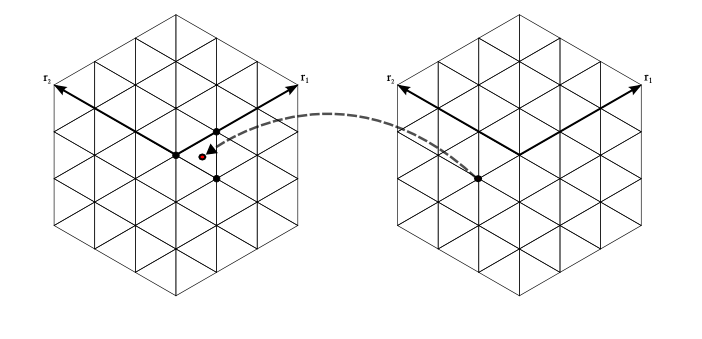
\includegraphics[scale=0.5]{figures/SL_hex.png} 
	\caption{Semi-Lagrangian step: Tracing back characteristics.}
	\label{fig:SL_hex}
\end{figure}


One of the advantages of the hexagonal mesh is its regularity. Indeed, even if the mesh is not Cartesian, localizing the characteristics' origin requires almost no computation. Let $(X_1, X_2)$ the Cartesian coordinates of the characteristics' origin, obtained by solving \eqref{eqn:charac_sys}. Then to obtain the hexagonal coordinates $(k_1, k_2)$ of the lowest point of the rhomboid encapsulating the point, we simply need to solve the system $\mathbf{x} = \mathbf{R} \mathbf{k}$, we get

\begin{equation}
	\label{eqn:k1k2}
	\left\lbrace
	\begin{array}{lclcl}
	k_1 &=&  \dfrac{\lfloor r_{22} X_1 - r_{21} X_2 \rfloor}{r_{11}*r_{22} - r_{12} r_{21}} & = &  \;\;\;\dfrac{1}{\sqrt{3}} X_1 + X_2\\[0.3cm]
	k_2 &=&  \dfrac{\lfloor r_{11} X_2 - r_{12} X_1 \rfloor}{r_{11}*r_{22} - r_{12} r_{21}} & = &  -\dfrac{1}{\sqrt{3}} X_1 + X_2
	\end{array}\right.
\end{equation}

After obtaining $(k_1, k_2)$, we know the rhomboid (composed by two cells) containing the characteristics' origin. To determine the exact cell on which the origin is located, we only need to verify if the abscissa of the point is greater than the abscissa of the mesh point at $(k_1, k_2)$ or not. In the first case the point belongs to the cell at the right, else to the cell at the left.


%%-----------------------------
\subsection{General Algorithm}

Below, we summarize the full algorithm to compute the distribution function $\rho^{n+1}$ solution of the non-constant advection equation \eqref{eqn:noncst_advec}.

\begin{description}
	\item[Initialization] At time $t=0$, we suppose that $\rho(\mathbf{x}, 0)$ is given.
	\item[Time Loop] Incrementation of a given time step $\Delta t$, such that: $t^{n+1} = t^n + \Delta t$
		\begin{itemize}
		\item Compute the \underline{characteristics' origins} using an ODE solver for \eqref{eqn:charac_sys};
		\item Interpolate the \underline{distribution function $\rho^n$} on that point using the mesh points in the vicinity;
		\item Update the known values: $\rho^n = \rho^{n+1}$.
		\end{itemize}
	\item[Remark] the boundary conditions will intervene in between the first and the second steps of the time loop (\emph{i.e.} before the interpolation step). On this paper we focus only on null Dirichlet boundary conditions.
\end{description}


\subsection{Time scheme}
We use a second order scheme which is the implicit Adams-Moulton scheme of order two: 

 \begin{equation*}
 	 \displaystyle{ \frac{\textbf{X}^{n+1}-\textbf{X}^{n}}{ \Delta t } =\frac{1}{2} ~( \textbf{A}^{n+1}+\textbf{A}^{n} ) }.
 \end{equation*} 
 
\noindent The difficulty here is that  $\textbf{A}(t^{n+1},\textbf{X}^{n+1})$ is unknown, thus an approximation $\overset{*}{\textbf{A}}$ of    $\textbf{A}$ at time $t^{n+1}$ is made thanks to previous computations:
 
 \begin{equation*}
\overset{*}{\textbf{A}}= 2~\textbf{A}(t^{n},\textbf{X}^{n+1}) -  \textbf{A}(t^{n-1},\textbf{X}^{n+1}).
 \end{equation*} 
 
\noindent The unknown $\textbf{X}^{n}$ is found by solving:
 
 
 \begin{equation*}
 	\begin{cases}
 	 \displaystyle{ \frac{\textbf{X}^{n+1}-\textbf{X}^{n}}{ \Delta t } =\frac{1}{2} ~(\overset{*}{\textbf{A}}+\textbf{A}^{n} ) },\\[3.5mm]
 	 \textbf{X}^{n+1}=\textbf{x}_i .
 	\end{cases}
 \end{equation*} 
 
A final remark: since we need $\textbf{A}(t^{n-1})$, the first step is done using the euler implicit time scheme. 
 
%%-----------------------------
%% Results
%%-----------------------------
\section{Numerical results}
\label{sec:results}
In this section we present the effectuated numerical simulations and their results. With the aim of studying the convergence, the dissipation, and the  efficiency of the methods, we first study the circular advection test case. To study the accuracy of the results, we compare them to a known solution. Then we proceed to the guiding-center simulation. As there is no model solution for this test case, we study properties of the system that we know should be conserved.


\subsection{Circular advection}

We focus here on the circular advection test case. The model is defined by:

	\begin{equation}
		\partial_t f(x,y,t) + y\,\partial_x f(x,y,t) - x \,\partial_y f(x,y,t) = 0 
	\end{equation}

As this equation is not coupled to Poisson model, we can study in detail the differences between the interpolation methods previously presented.	Additionally, finding the analytical solution is trivial and therefore we can study the convergence of our methods. Here, we take a Gaussian pulse as initial distribution function:

	\begin{equation}
	 f_0(x,y) = exp  \left( -\dfrac{1}{2} \left( \dfrac{(x - x_c)^2}{\sigma_x^2} + \dfrac{(y - y_c)^2}{\sigma_y^2  } \right)   \right ), 
	\end{equation}

On a hexagonal mesh centered at the origin, of radius $8$,  we take  $\sigma_x = \sigma_y = \frac{1}{2\sqrt{2}}$ (amplitude of the gaussian). Let us set here $x_c = 2$ and $y_c = 2$. The distance from the pulse to the limit of the domain makes the boundary effects negligeable, thus we can take a null Dirichlet boundary condition.  To study the convergence in space we took $N = 20, 40, 60, ..., 160$. We recall that $N$ is the number of cells on the radius $L$. With the maximum time of evaluation, $t_{max}$, at $6 \pi$, we chose to keep a constant CFL at $2$.



\begin{figure}[h!]
	\label{fig:circ_convergence}
	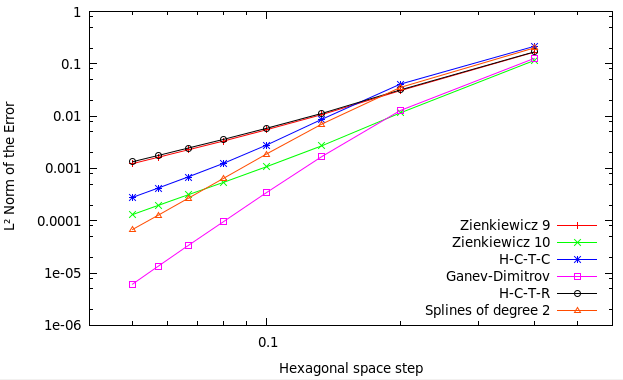
\includegraphics[width=0.45\textwidth]{figures/l2.png}
	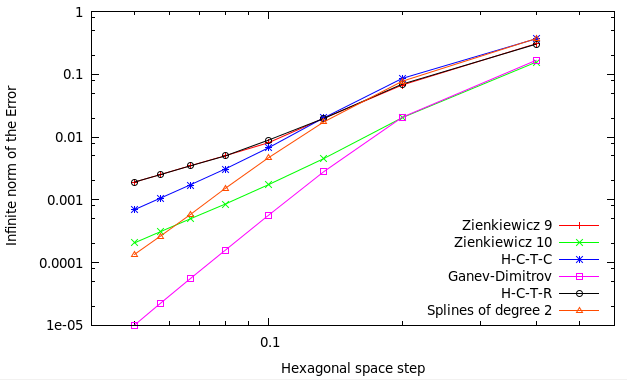
\includegraphics[width=0.45\textwidth]{figures/inf_l.png}
	\caption{Order of convergence}
\end{figure}

In Figure~\ref{fig:circ_convergence} we can see that for coarse meshes only the Ganev-Dimitrov method had a worst accuracy than the splines of degree $2$. Nonetheless, for finer grids, the splines obtain results better or as good as all the finite elements methods. Regarding the latter, we notice that there is little to no difference between Zienkiewicz-9 and the H-C-T-R method. 

\begin{figure}[h!]
	\label{fig:circ_performance}
	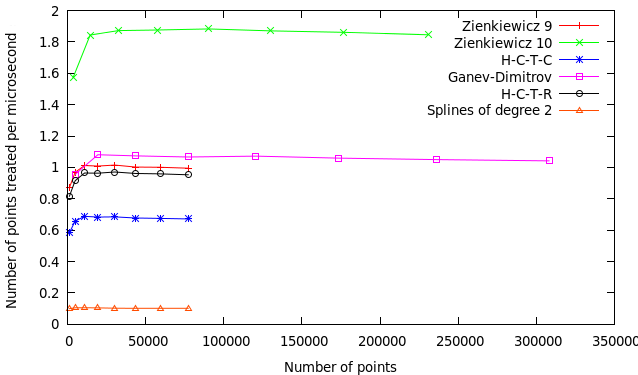
\includegraphics[scale=0.35]{figures/efficiency.png}
	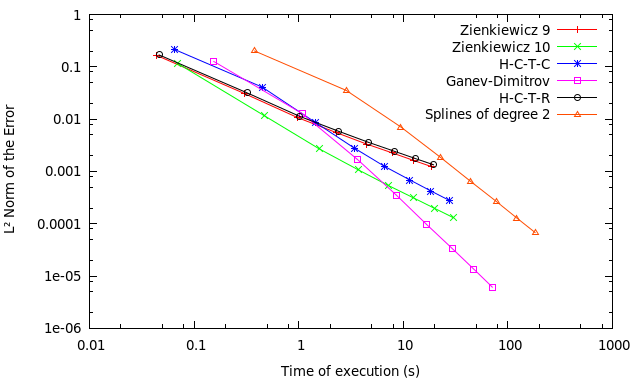
\includegraphics[scale=0.35]{figures/time_norm.png}
	\caption{Comparison of performances }
\end{figure}

Figure~\ref{fig:circ_performance} we can see that the level of performance of all the methods convergences quite quickly. It is also pretty obvious that even if the splines obtained more accuracy, the cost is more expensive than most of the Hermite Finite Element methods.

\subsection{Guiding-center model - Diocotron instability test case}


We consider here a guiding-center approximation of the 2D Vlasov-Poisson system, where the parallel velocity has been neglected and the magnetic field is set to $B = \begin{pmatrix} 0 & 0 & 1 \end{pmatrix}^T$. Furthermore, we consider the model in 2D in space and 1D in time. The reduced gyrokinetic model obtained\cite{filbet:hal-01068223} is

\begin{subnumcases}{\label{eqn:guiding_center}}
	\dfrac{\partial \rho}{\partial t} + E_{\perp} \cdot \nabla_{\mathbf{x}} \rho(\mathbf{x}, t) = 0\label{eqn:gc_vlasov}\\
	- \Delta \phi = \nabla \cdot E = \rho(\mathbf{x}, t) \label{eqn:gc_poisson}
\end{subnumcases}

with $E = (E_x, E_y) = - \nabla \phi $ and $E_\perp = (-E_y, E_x)$.

By neglecting the effect of boundary conditions, the  guiding center model verifies the following properties:
\begin{enumerate}
	\item Positivity of density $\rho$
 	\begin{equation*}
	 	 0\leq\rho(t,x,y).  
 	\end{equation*}
	\item Mass conservation
	\begin{equation*}
		\frac{d}{dt}\left(\int_{D}\rho dx dy\right)=0.
	\end{equation*}
	\item $L^p$ norm conservation, for $1\leq p\leq\infty$
	\begin{equation*}
		\frac{d}{dt}||\rho||_{L^p(D)}=0.
	\end{equation*}
	\item Energy conservation
	\begin{equation*}
		\frac{d}{dt}\left(\int_{D}|\nabla\phi|^2dx dy\right)=0.
	\end{equation*}
\end{enumerate}


This model, is commonly used in 2D simulations to study the particle density, as it describes highly magnetized plasmas in the poloidal plane of a tokamak.


We chose here to study the diocotron instability \cite{madaule:hal-00841504}.
The initial density is given by :
\begin{equation*}
 \rho_0(\mathbf{x}_\bot)=
 \left\{
 \begin{array}{ll}
  (1+\varepsilon\cos(\ell\theta))\exp{(-4(r-6.5)^2)},&\text{if  } r^-\leq\sqrt{x^2+y^2}\leq r^+,~ \text{with} ~\theta=\text{atan2}(y,x).\\[3mm]
  0,&\text{otherwise},
 \end{array}
 \right.
\end{equation*}
with $\theta=\text{atan2}(y,x)$.

\noindent As for the parameters, we take $\varepsilon=0.001$, $r^-=5$, $r^+=8$, $\ell=6$, furthermore $dt=0.1$ and the hexagonal step is $\frac{14}{160}$ with a radius of 14 and and an hexagonal parameter $nc =160$.
In this part, we won't test the Z3 approach as it requires a special resolution of the Poisson equation that has not been implemented. Indeed, computing the values of the field at the center of the triangles can't be combined with the resolution at the vertices. 
Moreover to even the commputational time of each method we chose to take $nc=80$ for the Ganev Dimitrov element as it results in the computations on a mesh with $nc =160$ ; see remark on the Ganev Dimitrov element in he paragraph on Hermite Finite element solver.\\
Let us note that 6 vortices is the main mode. If one takes $\ell\neq6$, but with epsilon small enough, one still sees the mode 6. With epsilon big enough, i.e. at least 0.1, the modes different from 6 can be visible for a time but they are not stable and we see the fusion or the apparition of vortices until there is the sixth mode. For instance,as illustrated by figure \ref{fig:mode9}, we can see the ninth mode turning into the sixth mode by fusion of vortices.

%\textcolor{red}{peut etre un paragraphe sur l'evolution de la densite, les 6 modes retrouves qqsoit eps, etc, commenter la figure 6}
\begin{figure}[h!]
	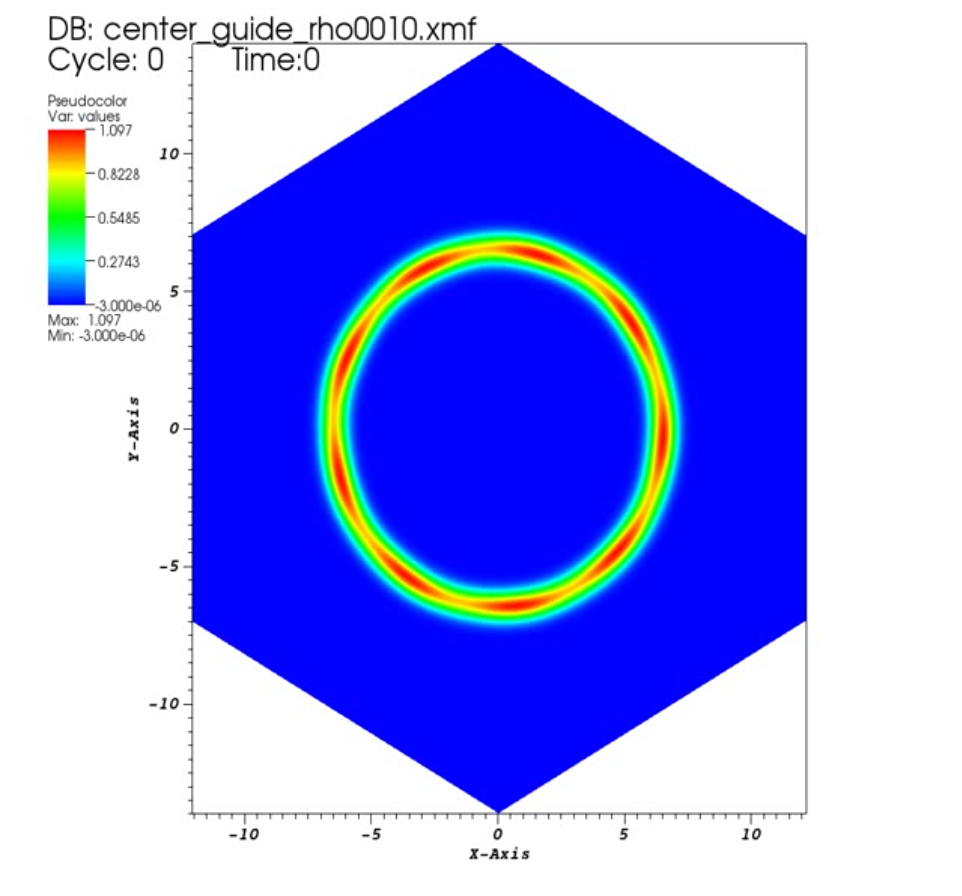
\includegraphics[width=0.3\textwidth]{figures/gc_spl_1.png}
	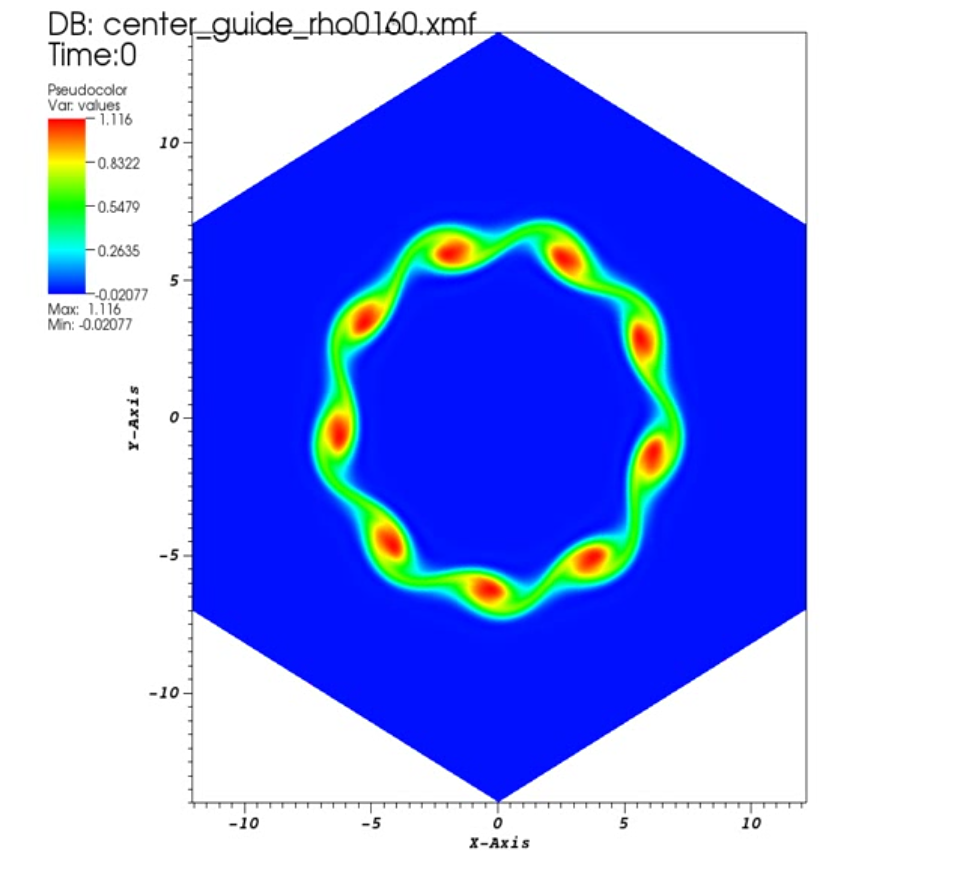
\includegraphics[width=0.3\textwidth]{figures/gc_spl_2.png}
	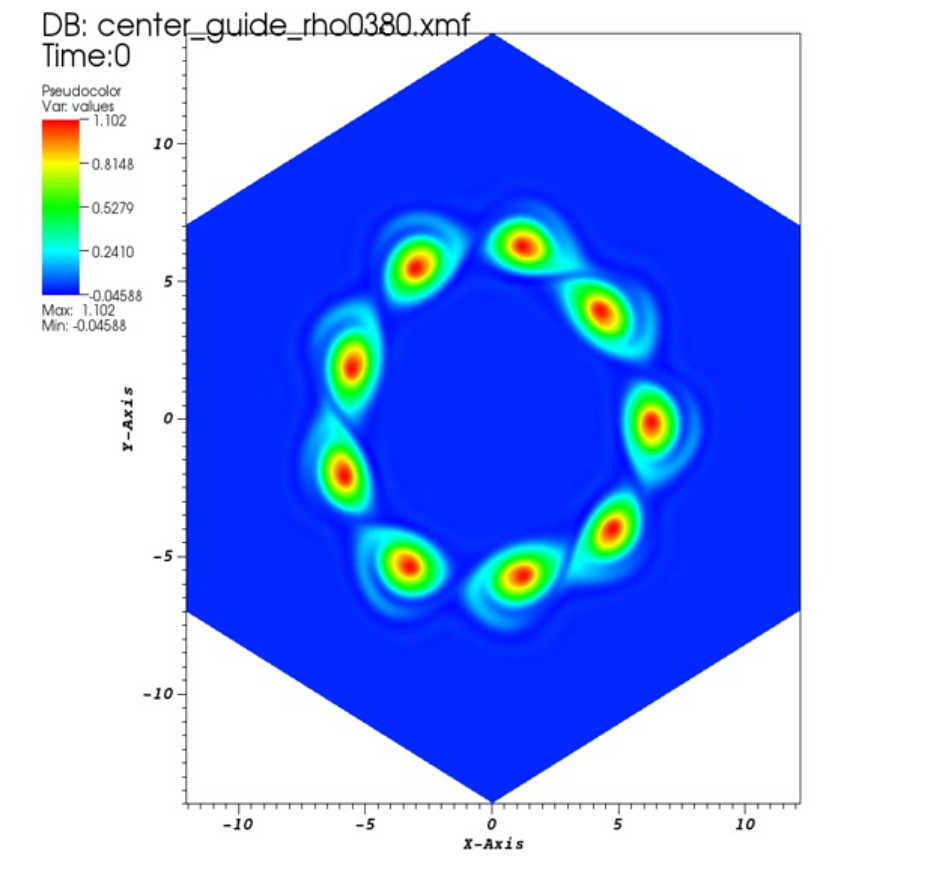
\includegraphics[width=0.3\textwidth]{figures/gc_spl_3.png}
	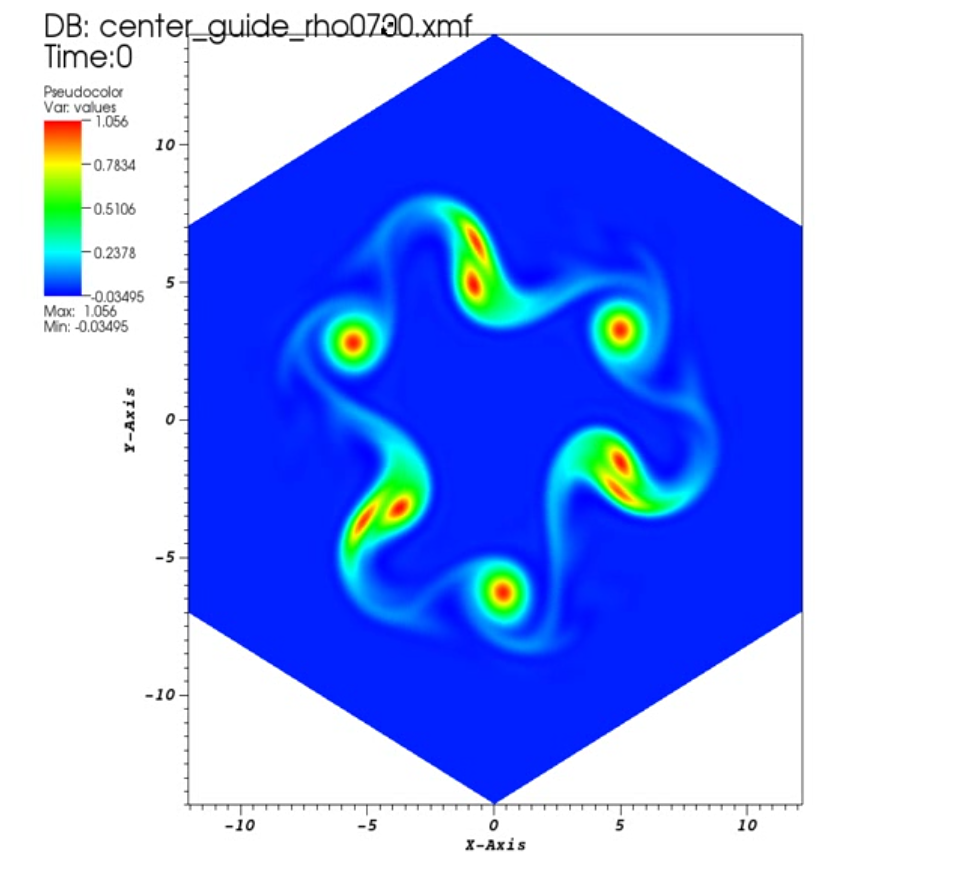
\includegraphics[width=0.3\textwidth]{figures/gc_spl_4.png}
	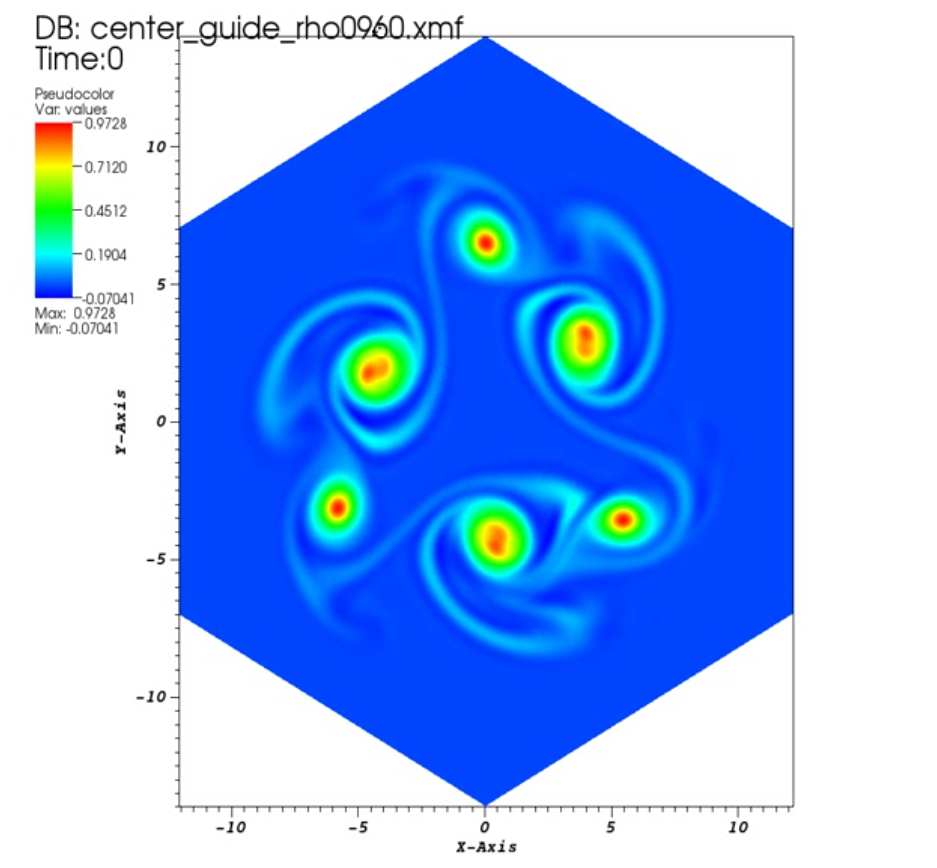
\includegraphics[width=0.3\textwidth]{figures/gc_spl_5.png}
	\caption{Time evolution of the guiding-center model, at times = }
	\label{fig:mode9} 
\end{figure}


Visualisation of the results. The six vortices are developping with time without losing any symetry. No obvious differences are visible on figure \ref{fig:comp_osci} to the naked eye which makes the diagnostics all the more important to compare the results computed.

%\begin{figure}[h!]
%	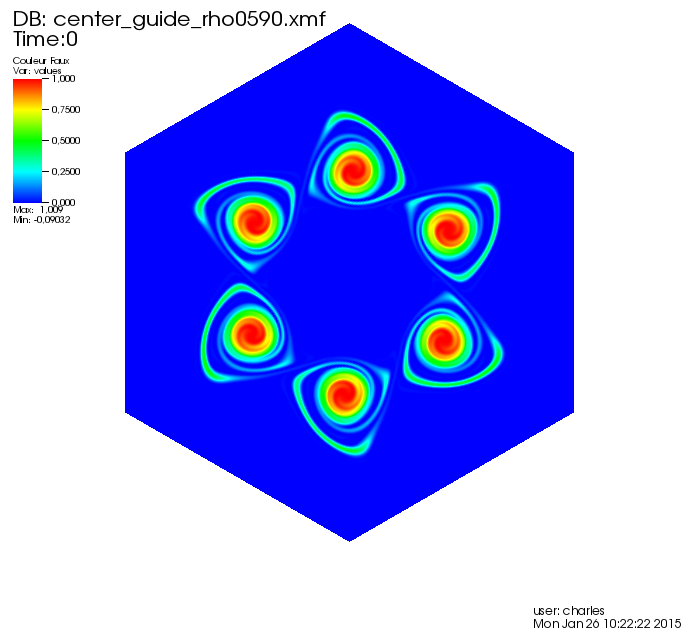
\includegraphics[width=0.35\textwidth]{figures/oscillations_hermite.png}
%	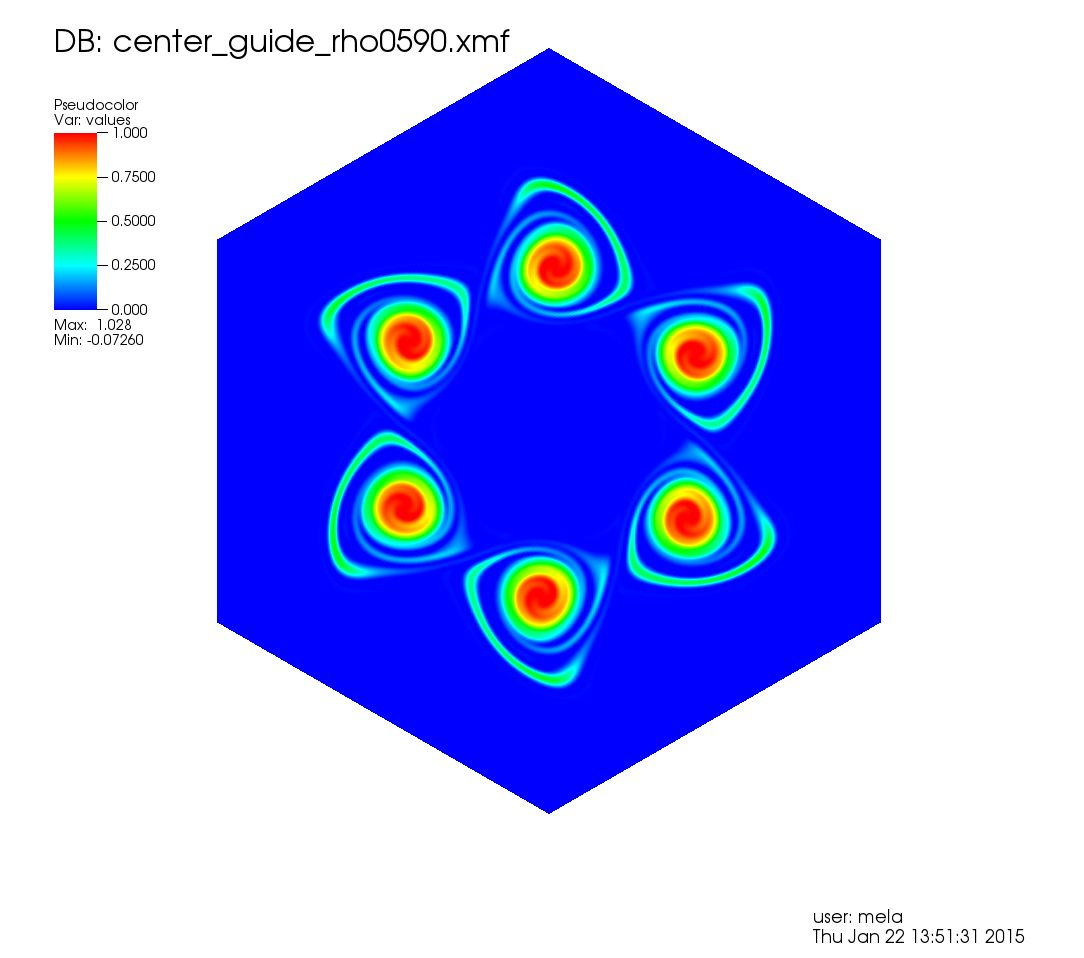
\includegraphics[width=0.35\textwidth]{figures/oscillations_splines.png}
%	\caption{\label{fig:comp_osci} Comparaison of oscillations: on the left with Hermite Finite Elements and on the right with splines}
%\end{figure}

\begin{figure}[h!]
	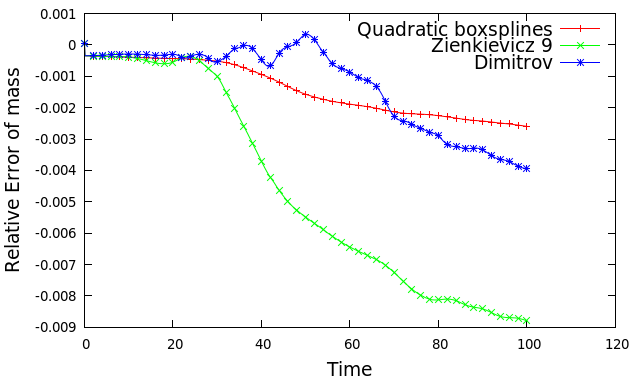
\includegraphics[scale=0.3]{figures/mass_cg.png}
	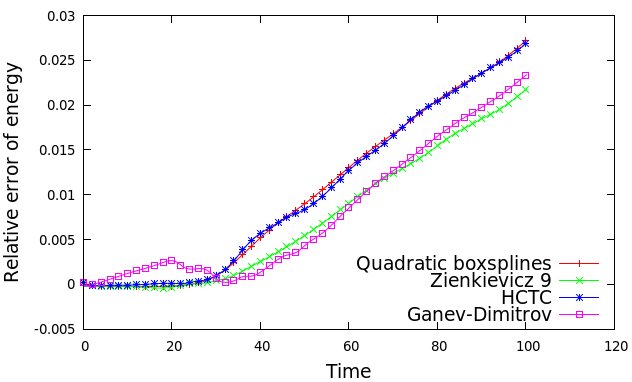
\includegraphics[scale=0.3]{figures/energy_cg.png}
	\caption{Time evolution of the relative error of mass and energy}
\end{figure}

\begin{figure}[h!]
	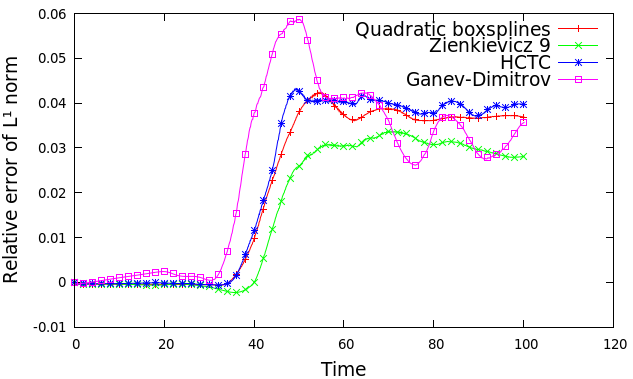
\includegraphics[scale=0.3]{figures/l1norm_cg.png}
	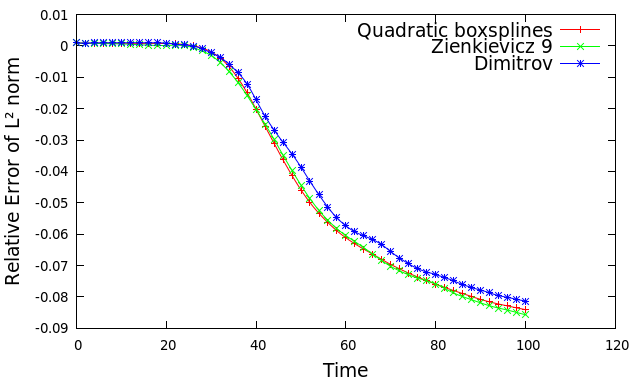
\includegraphics[scale=0.3]{figures/l2norm_cg.png}
	\caption{Relative error of $L^1$ and $L^2$ norms}
\end{figure}


\begin{figure}[h!]
	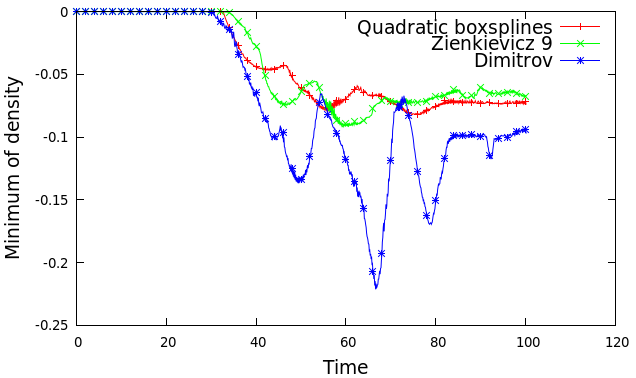
\includegraphics[scale=0.4]{figures/min_cg.png}
	\caption{Time evolution of the density's minimum}
\end{figure}
After comparison of the diagnostics we see that the various interpolation methods give close results overall. They are similar in terms of positivity conservation. One notices that if the box-splines conserve better the mass, the Z2 approach conserves better the $L^1$ norm. Also we note the box splines and the HCTC element give very near results whichever the diagnostic considered.  


%%-----------------------------
%% Conclusion
%%-----------------------------
\section{Conclusion}
\label{sec:conclusion}
In this paper we presented two Semi-Lagrangian schemes adapted to an hexagonal mesh. The strategies differentiated in the type of interpolation used: on the one hand, we developed an interpolation method based on box-splines --spline basis specific to the hexagonal mesh-- and on the other hand, we introduced an interpolation method based on Hermite Finite Elements. Furthermore, we presented a poisson solver based on finite differences on this mesh. The first simulations were made on the circular advection test case. This allowed to compare the order of the methods, as well as the efficiency. The splines approached seemed to be more accurate for finer grids, but a higher cost. Next, we simulated the 2D guiding-center model. The two method yield comparable results. Some minor differences could be observable when studying the mass conservation (where box-splines gave better results) and the conservation of the norms (where hermite finite elements yield more accurate solutions). Lastly, when comparing the densities, we perceived some noise, specially when working with Finite Elements.

%%-----------------------------
%%      your bibliography
%%-----------------------------

\newpage
\bibliographystyle{plain}
\bibliography{SelHex_proceedings.bib}

\end{document}

